\section{Background}
\label{sec:background}
\begin{figure}
    \centering
    \begin{subfigure}{0.45\textwidth}
    
\includegraphics[width=\textwidth]{figures/diffusion-orig.pdf}
    \end{subfigure}
    ~
    \begin{subfigure}{0.45\textwidth}
    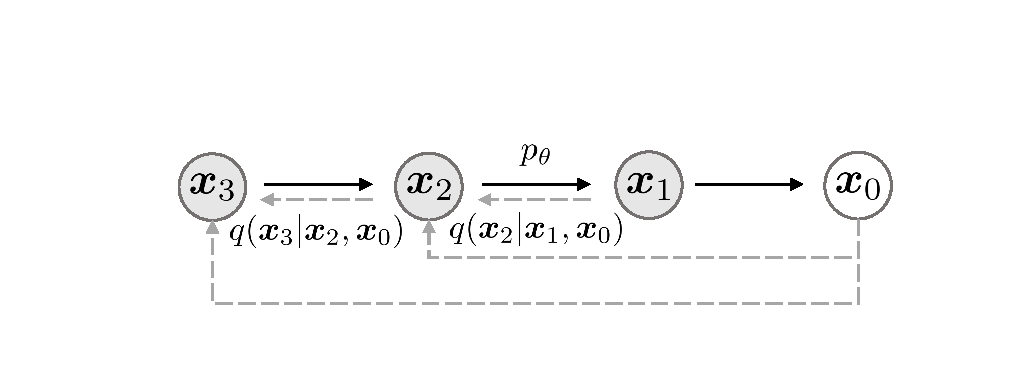
\includegraphics[width=\textwidth]{figures/diffusion-generalized.pdf}
    \end{subfigure}
    \caption{Graphical models for diffusion (left) and non-Markovian (right) inference models.}
    \label{fig:diffusion}
\end{figure}
Given samples from a data distribution $q(\bm{x}_0)$, we are interested in learning a model distribution $p_\theta(\bm{x}_0)$ that approximates $q(\bm{x}_0)$ and is easy to sample from. 
Denoising diffusion probabilistic models (DDPMs,~\citet{sohl-dickstein2015deep,ho2020denoising}) are latent variable models of the form
\begin{align}
    p_\theta(\bm{x}_0) = \int p_\theta(\bm{x}_{0:T}) \diff \bm{x}_{1:T}, \quad \text{where} \quad  p_\theta(\bm{x}_{0:T}) := p_\theta(\bm{x}_T) \prod_{t=1}^{T} p^{(t)}_\theta(\bm{x}_{t-1} | \bm{x}_t) \label{eq:gen}
\end{align}
where $\bm{x}_1, \ldots, \bm{x}_T$ are latent variables in the same sample space as $\bm{x}_0$ (denoted as $\gX$). The parameters $\theta$ are learned to fit the data distribution $q(\bm{x}_0)$ by maximizing a variational lower bound: %
\begin{align}
    \max_\theta \bb{E}_{q(\bm{x}_0)}[\log p_\theta(\bm{x}_0)] \leq \max_\theta \bb{E}_{q(\bm{x}_0, \bm{x}_1, \ldots, \bm{x}_T)}\left[\log p_\theta(\bm{x}_{0:T}) - \log q(\bm{x}_{1:T} | \bm{x}_0) \right] \label{eq:elbo}
\end{align}
where $q(\bm{x}_{1:T} | \bm{x}_0)$ is some inference distribution over the latent variables.
Unlike typical latent variable models (such as the variational autoencoder~\citep{rezende2014stochastic}), DDPMs are learned with a fixed (rather than trainable) inference procedure $q(\bm{x}_{1:T} | \bm{x}_0)$, 
and latent variables are relatively high dimensional. 
For example, \citet{ho2020denoising} considered the following Markov chain with Gaussian transitions 
parameterized by a decreasing sequence
$\alpha_{1:T} \in (0, 1]^T$:
\begin{align}
    q(\bm{x}_{1:T} | \bm{x}_0) := \prod_{t=1}^{T} q(\bm{x}_t | \bm{x}_{t-1}), \text{where} \ q(\bm{x}_t | \bm{x}_{t-1}) := \mathcal{N}\left(\sqrt{\frac{\alpha_t}{\alpha_{t-1}}} \bm{x}_{t-1}, \left(1 - \frac{\alpha_t}{\alpha_{t-1}}\right) \bm{I}\right) \label{eq:diff-ho}
\end{align}
where the covariance matrix is ensured to have positive terms on its diagonal.
This is called the \textit{forward process} due to the autoregressive nature of the sampling procedure (from $\bm{x}_0$ to $\bm{x}_T$). We call the latent variable model $p_\theta(\bm{x}_{0:T})$, which is a Markov chain that samples from $\bm{x}_T$ to $\bm{x}_0$, the \textit{generative process}, since it approximates the intractable \textit{reverse process} $q(\bm{x}_{t-1} | \bm{x}_t)$. Intuitively, the forward process progressively adds noise to the observation $\bm{x}_0$, whereas the generative process progressively denoises a noisy observation (\Figref{fig:diffusion}, left).

A special property of the forward process is that 
$$
q(\bm{x}_t | \bm{x}_0) := \int q(\bm{x}_{1:t} | \bm{x}_0) \diff \bm{x}_{1:(t-1)}= \mathcal{N}(\bm{x}_t; \sqrt{\alpha_t} \bm{x}_0, (1 - \alpha_t) \bm{I});
$$ 
so we can express $\bm{x}_t$ as a linear combination of $\bm{x}_0$ and a noise variable $\epsilon$:
\begin{align}
    \bm{x}_t = \sqrt{\alpha_t} \bm{x}_0 + \sqrt{1 - \alpha_t} \epsilon, \quad \text{where} \quad \epsilon \sim \mathcal{N}(\bm{0}, \bm{I}). \label{eq:reparam_xt}
\end{align}
When we set $\alpha_{T}$ sufficiently close to $0$, $q(\bm{x}_T | \bm{x}_0)$ converges to a standard Gaussian for all $\bm{x}_0$, so it is natural to set $p_\theta(\bm{x}_T) := \mathcal{N}(\bm{0}, \bm{I})$.
If all the conditionals %
are modeled as Gaussians with trainable mean functions and fixed variances, the objective in \eqref{eq:elbo} can be simplified to\footnote{Please refer to Appendix~\ref{app:ddpm} for details.}:
\begin{align}
    L_\gamma(\epsilon_\theta) & := \sum_{t=1}^{T}\gamma_t\bb{E}_{\bm{x}_0 \sim q(\bm{x}_0), \epsilon_t \sim \mathcal{N}(\bm{0}, \bm{I})}\left[  \norm{\epsilon_{\theta}^{(t)}(\sqrt{\alpha_t} \bm{x}_0 + \sqrt{1 - \alpha_t} \epsilon_t) - \epsilon_t}_2^2 \right] \label{eq:l-gamma}
\end{align}
where $\epsilon_\theta := \{\epsilon_\theta^{(t)}\}_{t=1}^{T}$ is a set of $T$ functions, each $\epsilon_{\theta}^{(t)}: \gX \to \gX$ (indexed by $t$) is a function with trainable parameters $\theta^{(t)}$, and $\gamma := [\gamma_1, \ldots, \gamma_T]$ is a vector of positive coefficients in the objective that depends on $\alpha_{1:T}$. 
In \citet{ho2020denoising}, the objective with $\gamma = \vone$ is optimized instead to maximize generation performance of the trained model; this is also the same objective used in noise conditional score networks~\citep{song2019generative} based on score matching~\citep{h2005estimation,vincent2011connection}. %
From a trained model, $\bm{x}_0$ is sampled by first sampling $\bm{x}_T$ from the prior $p_\theta(\bm{x}_T)$, and then sampling $\bm{x}_{t-1}$ from the generative processes iteratively. %


The length $T$ of the forward process is an important hyperparameter in DDPMs.
From a variational perspective, a large $T$ allows the reverse process to be close to a Gaussian~\citep{sohl-dickstein2015deep}, so that the generative process modeled with Gaussian conditional distributions becomes a good approximation; this motivates the choice of large $T$ values, such as $T = 1000$ in \citet{ho2020denoising}. %
However, as all $T$ iterations have to be performed sequentially, instead of in parallel, to obtain a sample $\bm{x}_0$, sampling from DDPMs is much slower than sampling from other deep generative models, which makes them impractical for tasks where compute is limited and latency is critical. %
